% Configuration

\documentclass[a4paper]{article}

\linespread{1.1}

\usepackage[utf8]{inputenc} 
\usepackage[T1]{fontenc}
\usepackage[francais]{babel}
\usepackage{amsmath}
\usepackage{amsfonts}
\usepackage{graphicx}
\usepackage{lmodern}
\usepackage{microtype}
\usepackage{hyperref}
\usepackage[margin=1.8cm]{geometry}
\usepackage{pgf,tikz}
\usepackage{mathrsfs}
\usetikzlibrary{arrows}


% Structure

\newcounter{c}
\newcounter{d}
\newcounter{r}
\newcounter{e}

\newcommand{\defi}{\subparagraph{D\'efinition \arabic{c}.\arabic{d} :}\stepcounter{d}}
\newcommand{\prop}{\subparagraph{Proposition \arabic{c}.\arabic{r} :}\stepcounter{r}}
\newcommand{\thm}{\subparagraph{Th\'eor\`eme \arabic{c}.\arabic{r} :}\stepcounter{r}}
\newcommand{\demo}{\subparagraph{D\'emonstration}}
\newcommand{\cor}{\subparagraph{Corollaire \arabic{c}.\arabic{r} :}\stepcounter{r}}
\newcommand{\lem}{\subparagraph{Lemme \arabic{c}.\arabic{r} :}\stepcounter{r}}
\newcommand{\rem}{\subparagraph{Remarque :}}
\newcommand{\chapitre}[1]{\stepcounter{c}\setcounter{e}{0}\setcounter{d}{0}\setcounter{r}{0}\noindent\textbf{\Large\arabic{c}. #1}\\}
\newcommand{\eq}[1]{\stepcounter{e}\begin{equation}#1\tag{\arabic{c}.\arabic{e}}\end{equation}}

% Notations

\newcommand{\Q}{\mathbb{Q}}
\newcommand{\Z}{\mathbb{Z}}
\newcommand{\N}{\mathbb{N}}
\newcommand{\R}{\mathbb{R}}
\newcommand{\C}{\mathbb{C}}
\newcommand{\E}[1]{\mathbb E\left(#1\right)}
\newcommand{\sph}{\mathbb{S}}
\newcommand{\p}{{\cal{P}}}
\newcommand{\fsp}{{\cal{F}}}
\newcommand*{\qed}{\hfill\ensuremath{\square}}
\newcommand{\x}{\mathbf x}
\newcommand{\y}{\mathbf y}
\newcommand{\e}{\mathbf e}
\newcommand{\scal}[2]{\langle#1,#2\rangle}
\newcommand{\trans}{^\text{T}\!}

\newcommand{\nor}[2]{{\cal N}(#1,#2)}
\newcommand{\mat}[2]{{\cal M}_{#1\times#2}(\R)}

\newcommand{\X}{\mathbf X}

\date{}
\author{Philippe Ricka}
\title{}

\begin{document}

This discussion is mainly based on slides 26 and 37 of Gerbeau's speech at VivaBrain summer school, June 29, 2017.

\bigskip 

\stepcounter{c}
\noindent{\Large\arabic{c} - Equations}
\bigskip

We consider a RCR network with current input $q(t)$ and total voltage $p(t)$. We note $R_1$ and $R_2$ the resistances and $C$ the capacitance. We also note $\pi$ the nodal pressure between the central connection and the ground.


We denote by $q_1,q_2$ and $q_C$ the current through the resistances and capacitance respectively.


\begin{center}
\begin{tikzpicture}
\draw (-1.7,0)--(-1.3,0);
\draw (1.3,0)--(1.7,0);
\draw (0,-1)--(0,-1.4);
\draw (-0.7,0)--(0.7,0);
\draw (0,0)--(0,-0.8);

% resistors
\draw (-1.3,0)--(-1.2,0.2)--(-1.1,-0.2)--(-1,0.2)--(-0.9,-0.2)--(-0.8,0.2)--(-0.7,0);
\draw (1.3,0)--(1.2,0.2)--(1.1,-0.2)--(1,0.2)--(0.9,-0.2)--(0.8,0.2)--(0.7,0);

% capacitor
\draw (-0.25,-0.8)--(0.25,-0.8);
\draw (-0.25,-1)--(0.25,-1);

% ground
\draw (-0.25,-1.4)--(0.25,-1.4);
\draw (-0.18,-1.45)--(0.18,-1.45);
\draw (-0.11,-1.5)--(0.11,-1.5);
\draw (-0.06,-1.55)--(0.06,-1.55);

\draw (1.7,0.25)--(1.7,-0.25);
\draw (1.75,0.18)--(1.75,-0.18);
\draw (1.8,0.11)--(1.8,-0.11);
\draw (1.85,0.06)--(1.85,-0.06);

% annotations
\draw (0,0) node [above] {$\pi$};

\draw (-1,0.3) node [above] {$R_1$};
\draw (1,0.3) node [above] {$R_2$};
\draw (0.3,-0.85) node [right] {$C$};

\draw[->] (-2.15,0)--(-1.75,0);
\draw (-2,0) node [above] {$p$};
\draw (-2,0) node [below] {$q$};

\end{tikzpicture}


~


$RCR~network$
\end{center}


The Kirschoff's law writes :

\eq{q_1=q_2+q_C}

From this relation, we can deduce an equation involving $\pi$ and $q=q_1$ :

\eq{q=\frac\pi{R_2}+C\frac{d\pi}{dt}}

we can rewrite, using $\pi=p-R_1q$ :

\eq{q=C\frac{dp}{dt}-CR_1\frac{dq}{dt}+\frac p{R_2}-\frac{R_1}{R_1}q}

resulting in :

\eq{C\frac{dp}{dt}+\frac p{R_1} = CR_1\frac{dq}{dt}+\left(1+\frac{R_1}{R_2}\right)q}


This last equation is the one used by J.F. Gerbeau, so his example is about input-to-ground pressure, and not about the node-to-ground one.


This looks like confirmed by the following simulation set run within Octave.

\bigskip 

\stepcounter{c}
\noindent{\Large\arabic{c} - Simulations}
\bigskip

As it is said in slide 37, we consider the inflow $q$ is given and generate synthetic pressure $p$.


The following two graphs are respectively the flow and pressure inputs computed using the Octave code reproduced at the end of this document. The inflow was recovered from Gerbeau's slide using WebPlotDigitizer (https://apps.automeris.io/wpd/), and compared with the function :

\eq{q(t)=10e^{-100(t-0.38)^2}+5}

The recovered plot and the plot of his function are very close to each other, and since the latter is smoother, we chose it to perform our calculations.


Since the plotted flow is in $cm^3s^{-1}$, we had to divide $q$ by $10^6$ to get $m^3s^{-1}$. The corresponding pressure was then computed in bar, so we divided it by $1.33332\times10^{-3}$ to get $Pa$.


The plots nicely fit with Gerbeau's ones.

\bigskip

Nevertheless, OpenModelica seems to give slightly different results that are to be discussed.

\begin{center}
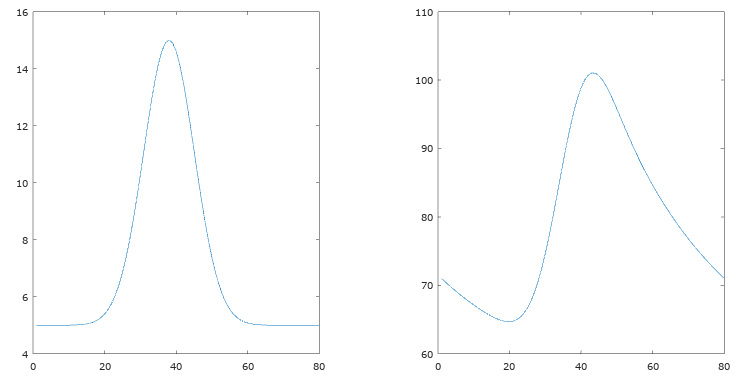
\includegraphics[width=\textwidth]{reprodGerbeau}
\end{center}

\bigskip

\stepcounter{c}
\noindent{\Large\arabic{c} - Octave}
\bigskip

\begin{verbatim}
clear
clf
format long

nloop = 5;
T = 0.8;
dt = 0.01;
C = 0.000025 ;
R1 = 1600;
R2 = 13000;
alpha = 1/(C/(dt) + 1/R2);
beta = 1 + R1/R2 + R1*C/(dt);
gamma = R1*C/(dt);

time = 1:T/dt;
q = (10*exp(-100*(time*dt-0.38).^2)+5)/1000000;
p = 0*time;

for i=1:nloop    
    for t=1:T/dt-1
        p(t+1) = alpha*(beta*q(t+1)-gamma*q(t)+C*p(t)/(dt));
    end
    p(1)=p(T/dt);
end

subplot(121)
plot(time,q*1000000)
subplot(122)
plot(time,100000*p/133.332)
\end{verbatim}

\end{document}